\documentclass[ openright,titlepage,numbers=noenddot,headinclude,twoside,%
                footinclude=true,cleardoublepage=empty,abstractoff,%
                BCOR=5mm,paper=a4,fontsize=11pt,%
                ngerman,american,%lockflag%
]{scrreprt}
\usepackage{graphicx}
\usepackage{amsmath}
\usepackage{fancyhdr}
\usepackage{braket}
\usepackage{modiagram}

\graphicspath{ {./Figures/} }

\pagestyle{fancy}
\lhead{jose-david creme}
\rhead{TODO 1}
\lfoot{TODO 1}
\rfoot{TODO 1}
%\def\changemargin#1#2{\list{}{\rightmargin#2\leftmargin#1}\item[]}
%\let\endchangemargin=\endlist
\title{Modeling properties of the double exchange model hamiltonian}

\begin{document}
\maketitle
\thispagestyle{fancy}
\chapter{Introduction}

Introduce the following topics
\begin{itemize}
  \item Colossal magnetic resistance
  \item Anomalous behavior of magnetic susceptibility in linear chain of Nickelates
\end{itemize}

\chapter{Double Exchange Hamiltonian}

The double exchange model is used to describe mixed valent transition
metal based molecules. The phenomenology of ferromagnetic and anti-ferromagnetic
behavior in such molecules is captured by the various parameters of the
double exchange model Hamiltonian (Eq:~\ref{eq:demodel}).

\begin{equation}
  \begin{split}
\hat{H} &= \sum_i 2K \hat{S}_{a_i}\cdot\hat{S}_{b_i} \\
        &+ \sum_{\braket{ij}} 2J_a \hat{S}_{a_i}\cdot\hat{S}_{a_j} \\
        &+ \sum_{\braket{ij}} t\left( \hat{c}^{\dagger}_{a_i}\cdot\hat{c}_{a_j} + \text{h.c.}\right ) \\
        &+ \sum_{i,i+1} V_{NN}\left ( \delta_{n_i,0}\ \delta_{n_{i+1},0} \right ) \\
        &+ \sum_{i,i+2} V_{NNN}\left ( \delta_{n_i,0}\ \delta_{n_{i+2},0} \right )
  \end{split}
\label{eq:demodel}
\end{equation}

The above Hamiltonian describes a model with two valence orbitals on each
atom (site) ideally of differnet symmetry (i.e. orthogonal, e.g. $a,b$). A schematic is shown in
Figure:~\ref{fig:deham}.

\begin{figure}[ht]
  \centering
\begin{modiagram}[names]
 \atom[$1$]{left}{
    1s = { 0; up} ,
    2s = { 1; up} ,
 }

 \atom[$2$]{right}{
    1s = { 0; up} ,
    2s = { 1;   } ,
 }
 \node[right,xshift=4mm] at (1sright) {$b$};
 \node[right,xshift=4mm] at (2sright) {$a$};
 \node[left,xshift=-4mm] at (1sleft) {$b$};
 \node[left,xshift=-4mm] at (2sleft) {$a$};
 \end{modiagram}
  \caption{\label{fig:deham} Schematic of the double exchange model with two valence orbitals on each atom.}
\end{figure}

The parameters in the model Hamiltonian are defined as follows:
\begin{itemize}

\item $K$ - The local exchange integral. This exchange integral represents
  Hund's rule and is always positive. The local exchange favors parallel
  coupling i.e. a local high spin determinant.

\item $J$ - The kinetic exchange interaction between type $a$

\end{itemize}

\section{Parameter Space}

Definition of the effective hamiltonian
Test changes


\chapter{Methodology}

\section{Exact diagonalization}

\section{Projector}

Introduce SLEPc and PETSc.

\section{Effective Hamiltonian}

\section{Real Space Renormalization Group}

\chapter{Results}

\section{Hole repulsion}

%TODO

\subsection{Weight vs J}
\subsubsection{Variation with Nsites}
\subsubsection{Variation with Repulsion}

\begin{figure}[ht]
    \centering
    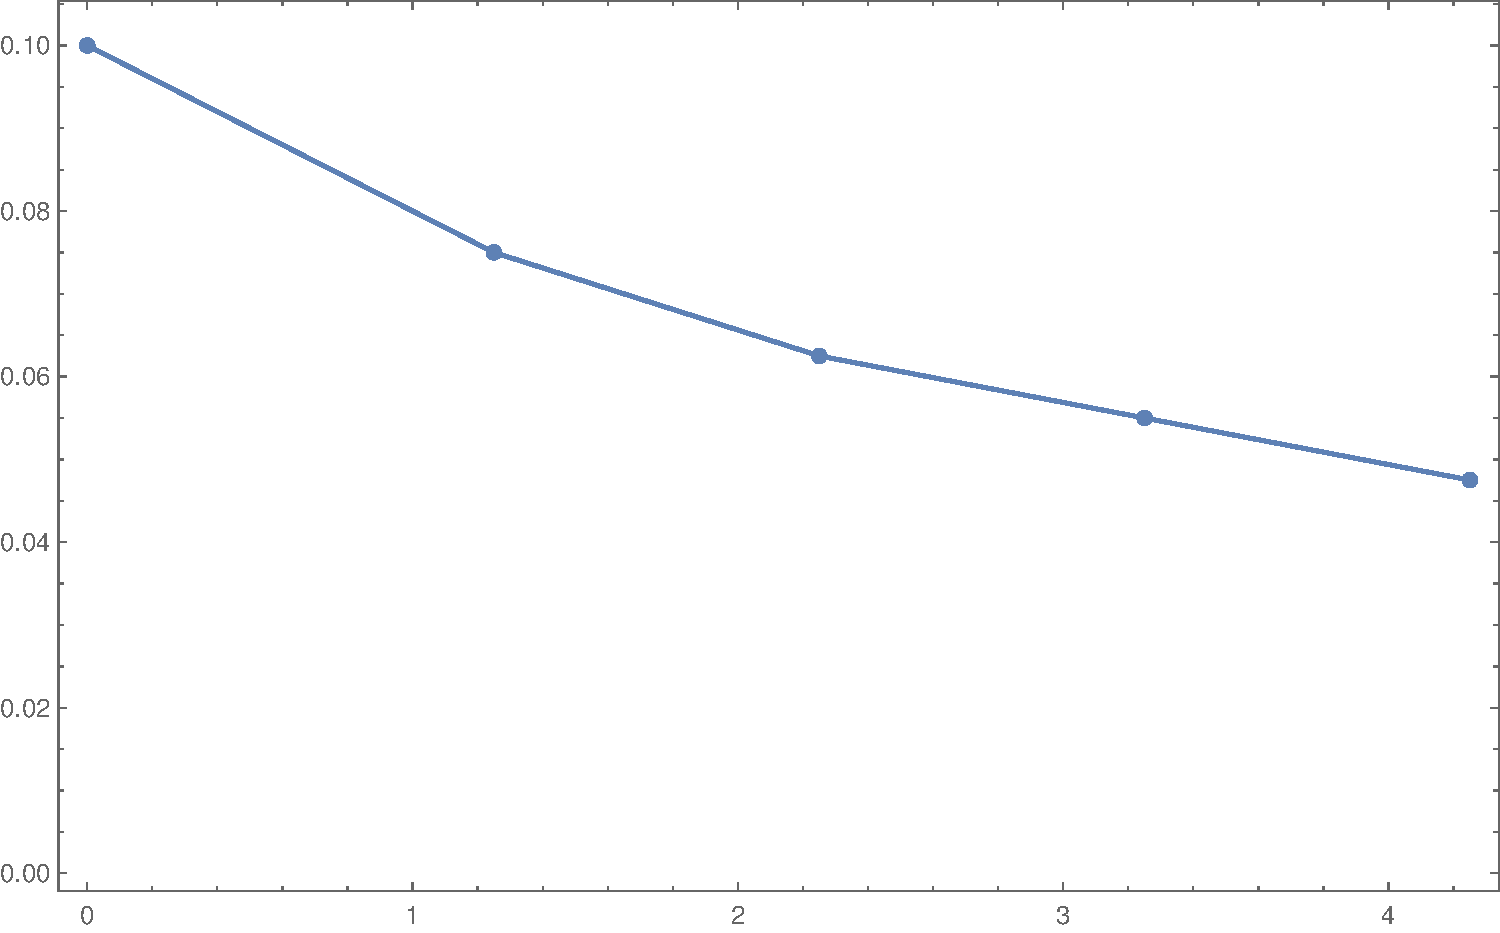
\includegraphics[scale=0.5]{12_4h_J_wmax_vs_xrep.pdf}
    \caption{\label{fig:}Variation of the value of $J$ for which we have a maximum in the weight vs the value of hole repulsion $V$. }
\end{figure}


\begin{figure}[ht]
    \centering
    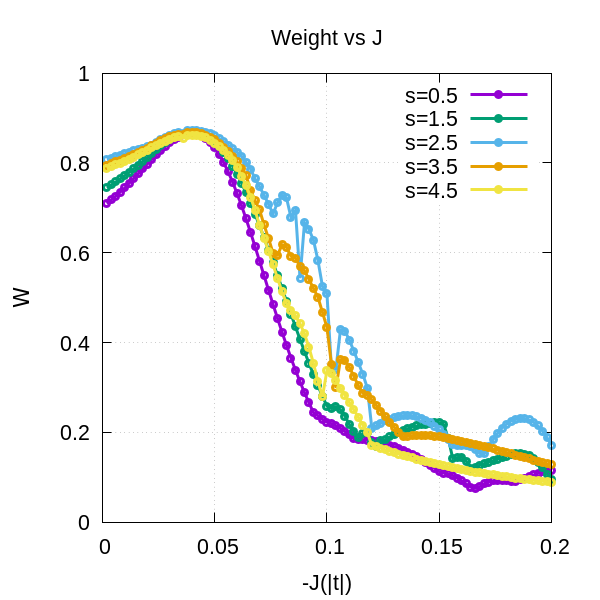
\includegraphics[scale=0.5]{Wmax_vs_J_xrep525.png}
    \caption{\label{fig:}Maximal weight as a function of J for xrep 525. }
\end{figure}

\subsection{$J_{eff}$ vs $J$}
\subsubsection{Variation with Nsites}
\subsubsection{Variation with Repulsion}

\subsection{RSRG}

\chapter{Discussion}

\chapter{Conclusion}

\end{document}



%*************************************************************************
% Bibliographies
%*************************************************************************
\addbibresource{biblio.bib}
